\documentclass[../dissertation.tex]{subfiles}

\begin{document}

\chapter{TD-Learning and Deep Reinforcement Learning for Importance Sampling Light Paths}

Monte Carlo Integration, importance sampling, Monte Carlo path tracing, reinforcement learning and the link between temporal difference learning and light transport have all been introduced. So now it is finally time to combine all of these concepts to build path tracing algorithms for Importance sampling. 

In this section I introduce two path tracers I have implemented to assess their ability in reducing image noise in Monte Carlo path tracing with a fixed number of sampled light paths per pixel. The first is based on a method introduced by Nvidia \cite{dahm2017learning} which I refer to as the Expected Sarsa path tracer. The other I refer to as the Neural-Q path tracer which I have designed. Both of which progressively reduce the number of zero-contribution light paths sampled during rendering, reducing the variance in the Monte Carlo approximation of a pixels colour. Ultimately, reducing the noise in rendered images. 

\section{The expected Sarsa Path Tracer}
\label{sec:expecte_sarsa_path_tracer}

The Expected Sarsa path tracer was first introduced by Nvidia \cite{dahm2017learning} to apply the derived  Expected Sarsa learning rule for learning the outgoing radiance in a given direction from a position, which was derived in \ref{eq:mc_expected_sarsa_td_learning}:

$$Q(x, \omega) \leftarrow (1 - \alpha) \cdot Q(x, \omega) + \alpha \cdot \left( L_e(y, -\omega) +\frac{2 \pi}{n} \sum_{k=1}^{n-1} Q(y, \omega_k) f_s(\omega_k, y, -\omega) \cos(\theta_k)  \right)$$

I will now introduce my implementation of the algorithm which uses it to progressively reduce the number of zero-contribution light paths sampled in a path tracer, which can reduce noise in rendered images significantly. 

\subsection{The Irradiance Volume}
The derived Expected Sarsa learning rule requires some sort of data-structure for looking up and updating the outgoing radiance at point $x$ in direction $\omega$, which from here on I will refer to as a Q-value. Therefore, the main requirement of the data structure is that it has some way of representing a discrete set of angles ($\omega_k$) in a hemisphere located at a position $x$ and oriented to the surface normal at $x$. The Irradiance Volume data structure \cite{greger1998irradiance} meets this requirement.\\

\begin{figure}[h]
\begin{center}
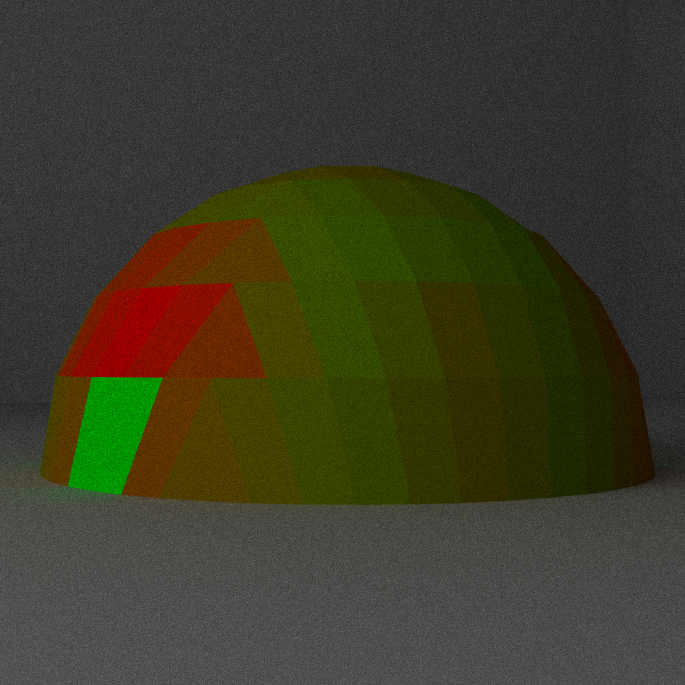
\includegraphics[width=0.3\textwidth]{images/renders/hemispheres/irradiance_volume.png}    
\end{center}
\caption{An Irradiance Volume. Each sector holds the incoming radiance $L_i(x,\omega_k)$, the more green a sector is the lower the stored radiance in that sector, the more red a sector is the higher the stored radiance in that sector. }
\label{fig:irradiance_volume}
\end{figure}

Originally designed to be used for pre-computation of radiance values which are looked up at runtime to approximate global illumination, the Irradiance Volume data structure is essentially a discretized version of a hemisphere which is visually represented in Figure \ref{fig:irradiance_volume}. The image shows the discrete sectors which make up a hemisphere, this was implemented by converting a 2D square grid into the 3D hemisphere shown, which is known as an adaptive quadrature. Where all sectors in the 2D grid have an equal area and a mapping introduced in \cite{shirley1994notes} converts the 2D grid coordinates into a regular discretized hemisphere in 3D space. The mapping ensures the hemisphere sectors remain equal to one another, meaning the discrete set of direction represented by the hemisphere are of equal angles apart from one another.\\

\begin{figure}[!htb]
\centering
\minipage{0.32\textwidth}
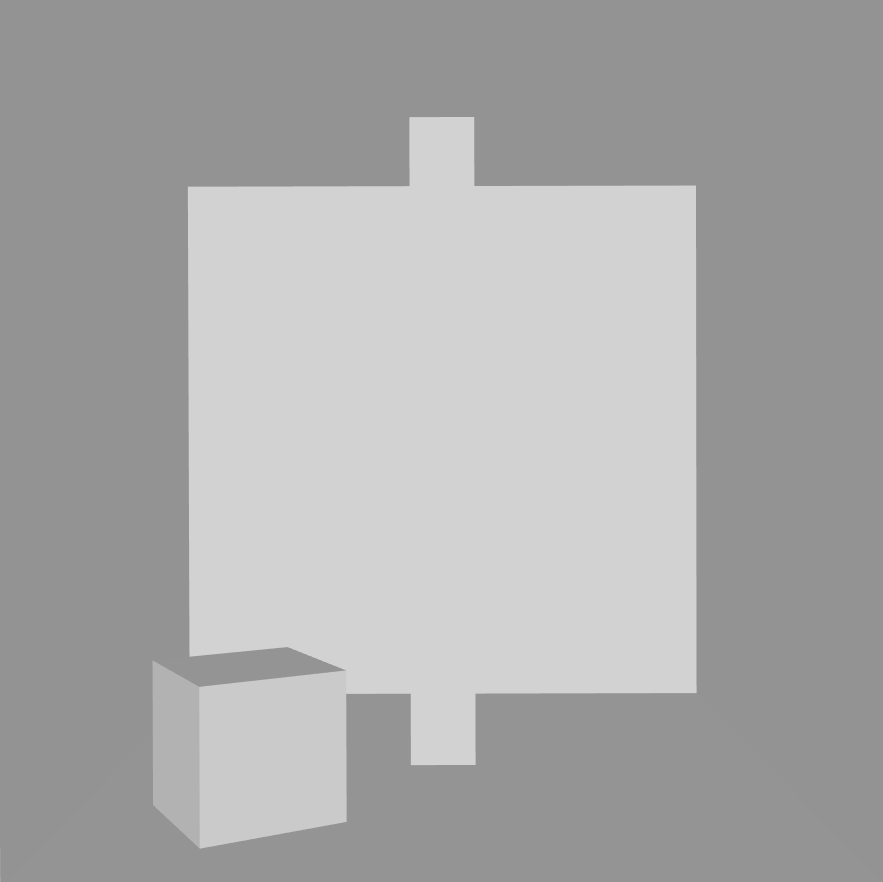
\includegraphics[width=1\textwidth]{images/renders/simple_room/geometry.png}
  \subcaption{Representation of the scenes geometry meshes}
\endminipage\hfill
\minipage{0.32\textwidth}
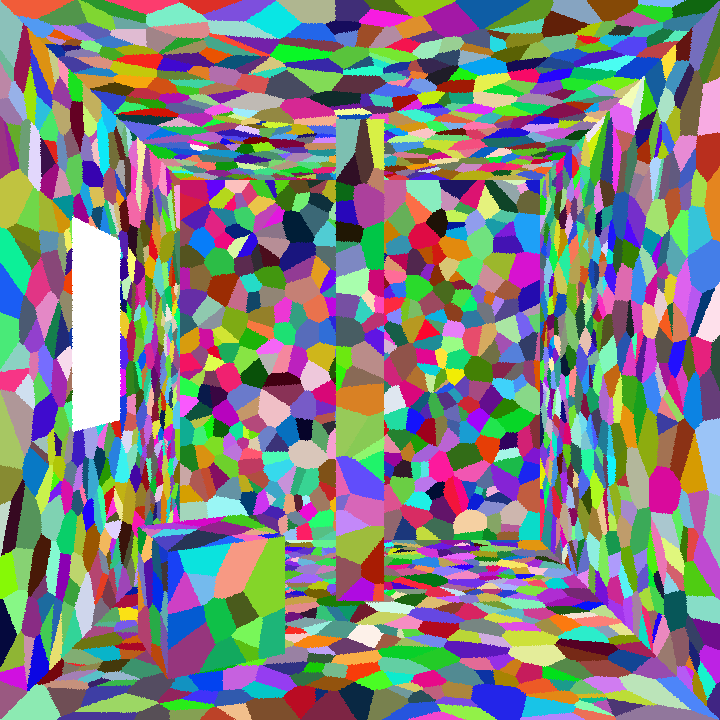
\includegraphics[width=1\textwidth]{images/renders/simple_room/voronoi.png}
   \subcaption{Voronoi Plot of Irradiance Volume locations}
\endminipage\hfill
\minipage{0.32\textwidth}
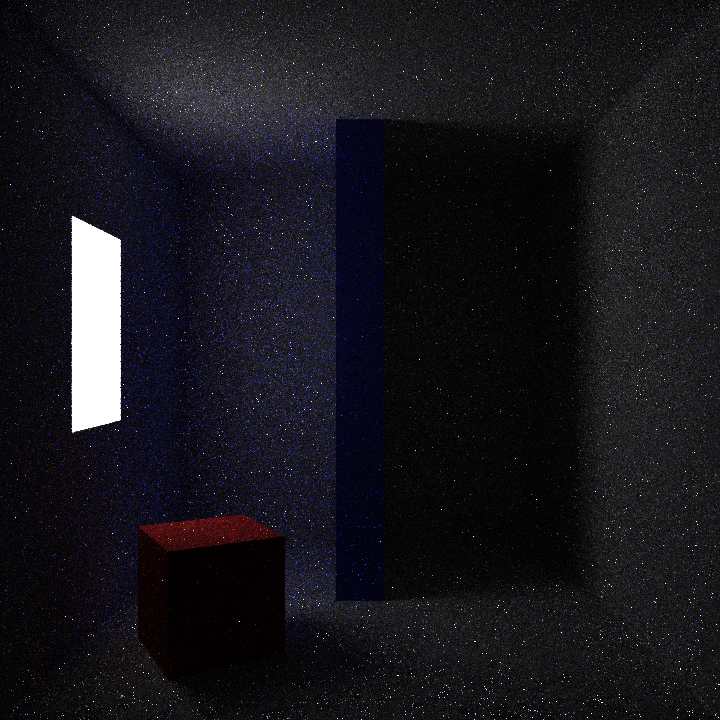
\includegraphics[width=1\textwidth]{images/renders/simple_room/reinforcement_16.png}
  \subcaption{Expected Sarsa path tracer with 16 SPP}
\endminipage
\caption{An example of discretizing location in the scene into Irradiance Volume locations. The geometry mesh (a) is used to uniformly sample Irradiance volume positions. Image (b) shows a voronoi plot for the Irradiance Volumes in the scene, where each pixel is coloured to the represent its closest Irradiance Volume, so each sector of colour in (b) represents a different Irradiance Volume location. Finally (c) gives a render using the Expected Sarsa path tracer based on Algorithm \ref{alg:expected_sarsa_pathtracer}.}
\label{fig:scene_discretization_example}
\end{figure}

Each sector of the Irradiance Volume is then used to store the current approximation of radiance from the centre of the hemispheres location $x$, in the outgoing direction formed by the unit vector from $x$ to the centre of the sector. Therefore, an Irradiance Volume stores the radiance (Q-value) for a given position $x$ (state) in each direction $\omega_k$ (action), for all sectors $k$ in the hemisphere located at $x$. In order to store Q-values across the scene, Irradiance Volumes can be uniformly sampled over the scenes geometry as shown in Figure \ref{fig:scene_discretization_example}. Then to lookup a radiance/Q-value for a given position $x$ in direction $\omega_k$, a nearest neighbour search is performed to find the closest Irradianc volume to position $x$, then retrieve the Q-value from the sector at index $k$. Giving a lookup and update time of $O(\log n) + O(1) = O(\log n)$ when using a data structure such as a KD-Tree for nearest neighbour search \cite{bentley1975multidimensional}. Lookup and update procedures from the Irradiance volumes in the scene is all that is needed to apply the Expected Sarsa learning rule in Equation \ref{eq:mc_expected_sarsa_td_learning}.

\subsection{Expected Sarsa Path Tracing}

\subsubsection{Algorithm}
The Expected Sarsa based path tracing algorithm is very similar to the original forward path tracer introduced in Algorithm \ref{alg:forward_path_tracing}. The algorithm learns online, meaning after every rendered frame pixel values are likely to have a lower variance due to a reduction in the number of zero contribution light paths. Initially radiance volumes are sampled uniformly across the room with all Q-values initialised to a small constant proportional to the number of sectors on each hemisphere $k$. This encodes the assumption that initially the radiance in all direction from any given point in the room is equal, as initially there is no prior knowledge of any radiance values $Q(x, \omega)$. With the radiance volumes set up, $n$ sampled light paths are traced through each pixel from the camera and into the scene. The average colour estimate of the $n$ sampled light paths per pixel is averaged to find the colour of each pixel, every rendered frame. The colour estimate of each sampled light path is found by Algorithm \ref{alg:expected_sarsa_pathtracer}. The two additions to this algorithm from the forward path tracer in Algorithm \ref{alg:forward_path_tracing}, are as follows:

\begin{enumerate}
\item Once the ray has intersected with a position in the scene $y$ from a position $x$, update the radiance estimate $Q(x, \omega)$ using the Expected Sarsa learning rule derived in Equation \ref{eq:mc_expected_sarsa_td_learning}. This is based on the light emitted from $y$ in direction $-\omega$ and the outgoing radiance estimate in direction $-\omega$ from point $y$ described by the summation. The summation involves summing all Q-values for the closest radiance volume to position $y$. Each of which are multiplied by BRDF of the surface at $y$, as well as the cosine of the angle between the sector direction for the Q-value ($\omega_k$) and the surface normal $y$.

\item The direction to continue the light path in is sampled proportional to the Q-values stored in the closest hemisphere to position $y$. This is achieved by normalizing the Q-values for the radiance volumes, converting them into a distribution which is appropriately known as the radiance distribution. Then inverse transform sampling \cite{devroye2006nonuniform} is performed to get a direction in the hemisphere to sample a ray in. Inverse transform sampling is where a random number $r \in [0,1]$ is sampled, then the largest number $x$ from the domain of the cumulative distribution $P(X)$ is returned where $ P(-\infty < X < x) \leq r$. 
\end{enumerate}

\begin{algorithm}[H]
\label{alg:expected_sarsa_pathtracer}
\SetKwProg{Fn}{Function}{ }{end}
\SetAlgoLined
 \Fn{pathTrace(camera, scene, pixel)}{  
   $throughput \leftarrow 1$\\
   $ray \leftarrow initialiseRayForPixel(pixel, camera)$\\
    \For{$i = 0$ \KwTo $\infty$}{
        $(y, norm) = closestIntersection(ray, scene)$\\
        \tcc{Addition (1)}
        \If{$i > 0$}{
            $Q(x, \omega) \leftarrow (1 - \alpha) \cdot Q(x, \omega) + \alpha \cdot \left( L_e(y, -\omega) +\frac{2 \pi}{n} \sum_{k=1}^{n-1} Q(y, \omega_k) f_s(\omega_k, y, -\omega) \cos(\theta_k)  \right)$
        }    
            
        \If{$noIntersection(y)$}{
            \Return $throughput \cdot \text{environmentLightRadiance}(ray,y)$
        }
        \ElseIf{$areaLightIntersection(y)$}{
            \Return $throughput \cdot \text{areaLightRadiance}(ray, y)$
        }
        \tcc{Addition (2)}
        $(\omega, \rho_i, f_s) \leftarrow \text{sampleRayDirProportionalToQ(y)}$\\
        $throughput \leftarrow throughput \cdot f_s \cdot cos(norm, \omega) / \rho_i$\\
        $ray \leftarrow (y,\omega)$
    }
 }
 \caption{Expected Sarsa forward path tracer \cite{dahm2017learning}}
\end{algorithm}

\subsubsection{Monte Carlo Integration}
It is important for the modified path tracing algorithm to converge to ensure consistency, meaning all introduced artefacts such as image noise are guarenteed to vanish over time \cite{dahm2017learning}. A decaying learning rate for $\alpha$ can be used to do so, see Equation \ref{eq:decay_lr}. Where $\text{i}(rv, \omega_k)$ is the number of times the rendering algorithm has updated the Q-value of the Irradiance Volume $i$ for sector $k$ representing angle $\omega_k$.

\begin{equation}
\label{eq:decay_lr}
\alpha(x, \omega) = \frac{1}{1 + \text{visits}(x, \omega_k)}
\end{equation}

Due to the importance sampling from addition (2), the probability density function over sampled directions $\omega$ at location $x$ is no longer uniform. Instead it is equal to the normalized Q-values for the closest Irradiance Volume to the point $x$. Therefore the evaluated probability density function $\rho_i$ must also take the shape of the probability distribution to correctly apply Monte Carlo Integration. To do so I have derived an Equation \ref{eq:mc_expected_sarsa_pdf} to determine the value $\rho_i$.

\begin{equation}
\label{eq:mc_expected_sarsa_pdf}
\rho_i = Q_p(x, \omega_k) \cdot n \cdot \frac{1}{2 \pi} = \frac{Q_p(x, \omega_k) \cdot n}{2 \pi}
\end{equation}

\noindent
Where:
\begin{conditions}
 Q_p(x, \omega_k)   & Normalized Q-value from the Irradiance Volume closest to $x$ at sector $k$\\
 n   & Total number of sectors in an Irradiance Volume \\
\end{conditions}

The reasoning behind this value $\rho_i$ is that $\frac{1}{2\pi}$ represents the probability density function ($pdf$) evaluated at any point when directions are randomly sampled in the hemisphere $\Omega$. However, the Irradiance Volume splits the hemisphere into discrete sectors, but each sector represents a continuous set of angles. Therefore if the probability of sampling a ray in each sector were constant $c$, $Q_p(x,\omega_k) = c$ $\forall k < n$, the $pdf$ would remain constant:

$$ \frac{Q_p(x, \omega_k) * n}{2\pi} = \frac{1}{2\pi}$$

However, the approximated radiance may vary across sectors, causing the associated $pdf$ to vary across sector due to $Q_p(x, \omega_k)$. This was not the case previously prior to importance sampling, where direction were sampled randomly over a unit hemisphere making a the $pdf$ is uniform. The diagram in Figure \ref{fig:pdfs} highlights these differences.

\begin{figure}[h]
\centering
\minipage{0.32\textwidth}
  
\includegraphics[width=\textwidth]{images/uniform_pdf.png}   
  \subcaption{Hemisphere with a uniform $pdf$}\label{fig:uniform_pdf}
\endminipage\hspace{5em}
\minipage{0.32\textwidth}
  
\includegraphics[width=\textwidth]{images/not_uniform_pdf.png}
  \subcaption{Irradiance Volume with a non-uniform $pdf$}\label{fig:not_uniform_pdf}
\endminipage
\caption{A 2 dimension view of a subset of values from two probability density functions ($pdf$). One for a unit hemisphere (left) with a uniform $pdf$. One for an Irradiance Volume (right) with non-uniform pdf. Where the arrows represent sampled directions and the values at the end are the evaluated $pdf$ values for each direction.}
\label{fig:pdfs}
\end{figure}

\subsubsection{Consistency}
While $Q(x, \omega_k)$ does converge, it does not necessarily converge on the true radiance $q_*(x, \omega_k)$. This is due to the discretization of the action/direction into sectors which make up a hemisphere. If the number of sectors was infinite then the algorithm would converge on the true radiance by the law of large number applied to Equation \ref{eq:mc_expected_sarsa_td_learning}. Clearly this is not possible, but later I discuss how increasing the number of  sectors on the Irradiance Volume affects the number of zero-contribution light paths. Another issue is Q-values will not be visited the same number of times during rendering. For example Irradiance Volumes located in places which are in the cameras view will be visited far more, so images rendered of the scene which have been in the cameras view for the longest are likely to have the lowest variance in pixel colours. This is a problem, as parts of the scene may look particularly noisy compared to others as the camera begins to move round the scene.

\pagebreak

% -----------------------------------------------------------------------------

\section{The Neural-Q Path Tracer}

Up to now I have only spoke of TD-learning techniques which involve use a tabular approach to approximate the the optimal value function (from section \ref{sec:optimal_value}, Equation \ref{eq:optimal_value}). However, it is possible to instead approximate the value function with a function approximater. Therefore I will introduce how a Neural Network can be used as a non-linear function approximater for the optimal value function \cite{deep_rl_function_approx}. Following this I introduce the Neural-Q path tracing algorithm I have designed and implemented.

After, I take a slight detour to review the new materials that have been recently published on neural networks for importance sampling in Monte Carlo path tracing. These materials were published during the execution of the project, so it is important to find out where my Neural Q-learning algorithm sits compared to these new state of the art methods.


\subsection{Introduction to Deep Reinforcement Learning}


\subsection{Neural-Q Path Tracer}


\subsection{Recent Advancements in Neural Light Path Construction}

\begin{comment}
% Advantages
% Less memory
% Same architecture can be applied to scene rather then applying complex data structures to the scene

Deep Learning for denoising light transport simulation rendering methods:
\begin{itemize}
\item \cite{zheng2018learning} - Uses a DNN to pre-train on a scene to figure out which pixels require more samples rather then just uniformly sampling the same amount of light rays for every pixel.

\item \cite{muller2018neural} - Uses a DNN for both online learning in light path construction and also introduces i for Primary Sample Space importance sampling. Performs well, not usable currently due to bottleneck of inference

"At any given point during rendering, a sample is generated by drawing a random pair u ∈ [0, 1] passing it through the inverted coupling layers in reverse order, and transforming to the range of cylindrical coordinates to obtain ω." - This means it simply gives a direction rather then return the value of directions around it, does this mean there is no stochasticity when sampling a new direction? Everytime we intersect with a world coordinate we will sample a ray in the same direction if no training occurs? Dont make this claim just allude to importance sampling over directions is better

\item \cite{keller2019integral} - Introduces a range of methods for NN, most related to mine is using NN to output Q-value of the light source.
\end{itemize}


{\bf A topic-specific chapter, of roughly $15$ pages} 
\vspace{1cm} 

\noindent
This chapter is intended to describe what you did: the goal is to explain
the main activity or activities, of any type, which constituted your work 
during the project.  The content is highly topic-specific, but for many 
projects it will make sense to split the chapter into two sections: one 
will discuss the design of something (e.g., some hardware or software, or 
an algorithm, or experiment), including any rationale or decisions made, 
and the other will discuss how this design was realised via some form of 
implementation.  

This is, of course, far from ideal for {\em many} project topics.  Some
situations which clearly require a different approach include:

\begin{itemize}
\item In a project where asymptotic analysis of some algorithm is the goal,
      there is no real ``design and implementation'' in a traditional sense
      even though the activity of analysis is clearly within the remit of
      this chapter.
\item In a project where analysis of some results is as major, or a more
      major goal than the implementation that produced them, it might be
      sensible to merge this chapter with the next one: the main activity 
      is such that discussion of the results cannot be viewed separately.
\end{itemize}

\noindent
Note that it is common to include evidence of ``best practice'' project 
management (e.g., use of version control, choice of programming language 
and so on).  Rather than simply a rote list, make sure any such content 
is useful and/or informative in some way: for example, if there was a 
decision to be made then explain the trade-offs and implications 
involved.

\section{Example Section}

This is an example section; 
the following content is auto-generated dummy text.
\lipsum

\subsection{Example Sub-section}

\begin{figure}[t]
\centering
foo
\caption{This is an example figure.}
\label{fig}
\end{figure}

\begin{table}[t]
\centering
\begin{tabular}{|cc|c|}
\hline
foo      & bar      & baz      \\
\hline
$0     $ & $0     $ & $0     $ \\
$1     $ & $1     $ & $1     $ \\
$\vdots$ & $\vdots$ & $\vdots$ \\
$9     $ & $9     $ & $9     $ \\
\hline
\end{tabular}
\caption{This is an example table.}
\label{tab}
\end{table}

\begin{algorithm}[t]
\For{$i=0$ {\bf upto} $n$}{
  $t_i \leftarrow 0$\;
}
\caption{This is an example algorithm.}
\label{alg}
\end{algorithm}

\begin{lstlisting}[float={t},caption={This is an example listing.},label={lst},language=C]
for( i = 0; i < n; i++ ) {
  t[ i ] = 0;
}
\end{lstlisting}

This is an example sub-section;
the following content is auto-generated dummy text.
Notice the examples in Figure~\ref{fig}, Table~\ref{tab}, Algorithm~\ref{alg}
and Listing~\ref{lst}.
\lipsum

\subsubsection{Example Sub-sub-section}

This is an example sub-sub-section;
the following content is auto-generated dummy text.
\lipsum

\paragraph{Example paragraph.}

This is an example paragraph; note the trailing full-stop in the title,
which is intended to ensure it does not run into the text.


\subsection{Plan}

% I imagine this section to be like a mini paper starting at new method

\textbf{Breakdown}
\begin{enumerate}

\item State learning rule for deep Q-learning and the difference from deep Q-learning to q-learning. Maybe some of the difficulties associated with deep q-learning versus q-learning, and some of the general advantages. 

\item Derive the learning rule for deep q-learning network which I used, once again justifying terms throughout the derivation.

\item Explain concept of eta-greedy policy used. Explain exploration vs exploitation but we will talk about this more later

\item Describe how the current method is used for diffuse surfaces. Introduce the pseudo code for the new algorithm. Give a description of each stage and what it does. Relating back to properties such as bias rendering and pointing out assumption made by the path tracer.

\item Present and explain the network architecture. Explain in depth about how the state was modelled as a point relative to all vertices to give the network information about the position of the vertex relative to the rest of the world compared to passing in a single position. Relate this to Atari games, we get an image showing where we are relative to the world rather than just a single position in the world.

\item Present some results side by side against a default path tracer and Nvidia's reinforcement learning approach. Pointing out aspects of the image and reasoning for certain parts.

\end{enumerate}
\end{comment}

\end{document}